%=============================================================================
%  SolveBench -- Direct vs. Iterative Linear Solvers on Real Engineering Data
%  CSE 402 Project Proposal -- 5-minute pitch, 4-slide deck
%  Compile with pdflatex
%=============================================================================
\documentclass[aspectratio=169,10pt]{beamer}

\usepackage[utf8]{inputenc}
\usepackage[T1]{fontenc}
\usepackage{lmodern}
\usepackage[scaled=0.92]{helvet}
\renewcommand{\familydefault}{\sfdefault}
\usepackage{amsmath,amssymb}
\usepackage{booktabs}
\usepackage{array}
\usepackage{colortbl}
\usepackage{graphicx}
\usepackage{pifont}
\usepackage{tikz}
\usetikzlibrary{arrows.meta,positioning,shapes.geometric,calc,fit,backgrounds}

%------------------------------------------------ EDIT ME: group details
\newcommand{\memberOne}{2105037}
\newcommand{\memberTwo}{2105038}
\newcommand{\memberThree}{2105042}
\newcommand{\memberFour}{2105047}
\newcommand{\memberFive}{2105054}

%------------------------------------------------ palette
\definecolor{LSnavy}{RGB}{15,52,80}
\definecolor{LSteal}{RGB}{18,110,120}
\definecolor{LSgold}{RGB}{193,138,52}
\definecolor{LSgreen}{RGB}{40,120,86}
\definecolor{LSred}{RGB}{176,58,58}
\definecolor{LSbg}{RGB}{252,251,248}
\definecolor{LSgray}{RGB}{92,100,108}
\definecolor{LSlight}{RGB}{234,240,240}
\definecolor{LSlightgold}{RGB}{247,241,229}

%------------------------------------------------ beamer look & feel
\usetheme{default}
\setbeamertemplate{navigation symbols}{}
\setbeamercolor{background canvas}{bg=LSbg}
\setbeamercolor{normal text}{fg=LSnavy}
\setbeamercolor{structure}{fg=LSteal}
\setbeamercolor{frametitle}{fg=LSnavy,bg=LSbg}
\setbeamercolor{title}{fg=LSnavy}
\setbeamercolor{itemize item}{fg=LSteal}
\setbeamercolor{itemize subitem}{fg=LSgold}
\setbeamercolor{block title}{fg=white,bg=LSteal}
\setbeamercolor{block body}{fg=LSnavy,bg=LSlight}

\setbeamerfont{frametitle}{series=\bfseries,size=\large}
\setbeamerfont{title}{series=\bfseries,size=\Large}
\setbeamerfont{block title}{series=\bfseries}
\setbeamertemplate{itemize item}{\small\raise0.15ex\hbox{\ding{110}}}
\setbeamertemplate{itemize subitem}{\footnotesize\raise0.1ex\hbox{\ding{119}}}

\setbeamertemplate{frametitle}{%
  \vspace{0.55em}%
  \begin{beamercolorbox}[wd=\paperwidth,leftskip=0.9cm,rightskip=0.9cm]{frametitle}%
    \strut\insertframetitle\strut\par
    {\color{LSteal}\rule{0.55\linewidth}{1.4pt}}%
    {\color{LSgold}\rule{0.10\linewidth}{1.4pt}}%
  \end{beamercolorbox}%
}

\setbeamertemplate{footline}{%
  \hbox{%
    \begin{beamercolorbox}[wd=.36\paperwidth,ht=2.4ex,dp=1.1ex,leftskip=0.9cm]{}%
      {\color{LSgray}\scriptsize SolveBench}\hfill%
    \end{beamercolorbox}%
    \begin{beamercolorbox}[wd=.44\paperwidth,ht=2.4ex,dp=1.1ex,center]{}%
      {\color{LSgray}\scriptsize CSE 402 Project Proposal}%
    \end{beamercolorbox}%
    \begin{beamercolorbox}[wd=.20\paperwidth,ht=2.4ex,dp=1.1ex,rightskip=0.9cm]{}%
      \hfill{\color{LSteal}\scriptsize\bfseries\insertframenumber}%
    \end{beamercolorbox}%
  }\vspace{1pt}%
}

%------------------------------------------------ macros
\renewcommand{\emph}[1]{{\color{LSteal}\bfseries #1}}
\newcommand{\gd}[1]{{\color{LSgreen}\bfseries #1}}
\newcommand{\hdrow}{\rowcolor{LSnavy}}
\newcommand{\hdtxt}[1]{\textcolor{white}{\bfseries #1}}

% shared tikz styles for the pipeline diagram
\tikzset{
  stage/.style={rounded corners=3pt,draw=LSteal,line width=1pt,fill=LSlight,
                text=LSnavy,align=center,inner sep=6pt,font=\footnotesize\bfseries},
  data/.style={rounded corners=3pt,draw=LSgold,line width=1pt,fill=LSlightgold,
               text=LSnavy,align=center,inner sep=6pt,font=\footnotesize},
  outbox/.style={rounded corners=3pt,draw=LSgreen,line width=1.2pt,fill=LSlightgold,
               text=LSnavy,align=center,inner sep=6pt,font=\footnotesize\bfseries},
  fl/.style={-{Stealth[length=2.6mm]},line width=1.1pt,draw=LSteal},
}
\newcommand{\subtag}[1]{\\{\scriptsize\color{LSgray}\normalfont #1}}

%=============================================================================
\title{SolveBench}
\subtitle{Direct vs. Iterative Linear Solvers on Real Power-Grid \& Structural Systems}
\date{}
%=============================================================================
\begin{document}

%----------------------------------------------------------------- TITLE
\begin{frame}[plain]
  \begin{tikzpicture}[remember picture,overlay]
    \fill[LSnavy] (current page.south west) rectangle ([yshift=2.0cm]current page.south east);
    \node[anchor=west] at ([yshift=1.0cm,xshift=0.9cm]current page.south west)
      {\color{LSgold}\footnotesize\bfseries Section A2 $\cdot$ Roll Numbers \;\;
       \color{LSlight}\normalfont \memberOne\ $\cdot$ \memberTwo\ $\cdot$ \memberThree\ $\cdot$ \memberFour\ $\cdot$ \memberFive};
    \fill[LSgold] ([yshift=7.86cm,xshift=0.92cm]current page.south west) rectangle
                  ([yshift=7.72cm,xshift=2.5cm]current page.south west);
  \end{tikzpicture}
  \vspace{1.0cm}
  \hspace{0.4cm}%
  \begin{minipage}{0.94\linewidth}
    {\color{LSteal}\bfseries\large SOLVEBENCH}\\[0.45em]
    {\color{LSnavy}\fontsize{28}{32}\selectfont\bfseries Solving $A\vec{x}=\vec{b}$ at Scale}\\[0.3em]
    {\color{LSnavy}\Large Direct vs.\ Iterative Solvers \& Our Novel APK Method}\\[0.85em]
    {\color{LSgray}\normalsize Every blackout-prevention study and every bridge safety check
     reduces to this exact equation. We benchmark classical solvers against our proposed method.}
  \end{minipage}
\end{frame}

%----------------------------------------------------------------- BASE PAPER
\begin{frame}{Base Paper: What It Studies}
  \vspace{-0.15em}
  \colorbox{LSlight}{\parbox{0.98\linewidth}{\vspace{0.2em}
    {\bfseries\normalsize\color{LSnavy} ``Comparative Analysis of Jacobi and Gauss-Seidel Iterative Methods''}\\[0.18em]
    {\footnotesize\color{LSgray} P.\ Khrapov and N.\ Volkov}\\[0.12em]
    {\footnotesize\color{LSteal}\emph{International Journal of Open Information Technologies}, vol.\ 12, no.\ 2, pp.\ 23--34, 2024}\\[0.2em]
    {\footnotesize\color{LSgray}\textbf{Domain:} Numerical linear algebra, iterative methods for
    solving systems of linear algebraic equations (SLAEs).}
    \vspace{0.2em}}}
  \vspace{0.25em}
  \small
  \begin{itemize}\setlength\itemsep{0.2em}
    \item \textbf{Maps out exactly} which matrices make the Jacobi and
      Gauss-Seidel methods converge, by tracking where the roots of a
      characteristic polynomial fall inside the unit circle, either directly
      or via a \textbf{Hurwitz-style stability test}.
    \item Proves this exactly, by hand, for \textbf{2 and 3 unknowns} (both
      complex and real coefficients), then checks the same pattern
      \textbf{statistically with code} across 100{,}000 randomly generated
      matrices, up to 5 unknowns.
    \item Shows the two methods do \emph{not} always share the same convergence
      region: \emph{which} method wins depends on the structure of the matrix.
  \end{itemize}
  \vspace{0.25em}
  \begin{block}{\small The gap this leaves open}
    \footnotesize The analysis stops at toy systems of \textbf{5 unknowns or fewer}
    and only two solvers. Real engineering systems have \textbf{thousands} of
    unknowns. Nobody in the paper tests these convergence claims on real data.
  \end{block}
\end{frame}

%----------------------------------------------------------------- PROBLEM & SCOPE
\begin{frame}{Problem Statement \& Scope}
  \small
  \textbf{Problem:} every real engineering simulation, whether it's modeling
  a power grid, checking a structure's safety, or simulating a circuit,
  comes down to the same core step: solving $A\vec{x}=\vec{b}$. Get the
  solver choice wrong, and what should take milliseconds either \gd{crawls}
  or \textcolor{LSred}{\bfseries never converges}.

  \vspace{0.5em}
  \begin{center}
  \colorbox{LSlightgold}{\parbox{0.92\linewidth}{\centering\footnotesize
  \textbf{Category: Exploratory \& Comparative Study.} We benchmark eight
  classical direct and iterative solvers against real, not synthetic,
  engineering data.}}
  \end{center}

  \vspace{0.7em}
  \renewcommand{\arraystretch}{1.3}
  \begin{tabular}{@{}p{2.9cm}p{1.5cm}p{2.0cm}p{5.0cm}@{}}
    \toprule
    \hdrow \hdtxt{Domain} & \hdtxt{Systems} & \hdtxt{Size range} & \hdtxt{Real-world meaning}\\
    \midrule
    Power-grid admittance & 11 & 118 to 1{,}723 buses & The linear system solved every
      time a utility models its own grid.\\
    \rowcolor{LSlight}
    Structural (stiffness \& mass) & 33 & 112 to 4{,}884 DOF & The linear system solved to check
      if a real building or bridge design holds.\\
    Circuit simulation & 4 & 2{,}624 to 5{,}860 nodes & The linear system solved
      at every timestep of a transient circuit simulation.\\
    \bottomrule
  \end{tabular}

  \vspace{0.6em}
  \footnotesize\color{LSgray}
  48 real matrices spanning three engineering domains, two to three orders of
  magnitude beyond the base paper's own 5-unknown ceiling, drawn from a
  2{,}904-matrix collection with room to scale further.
\end{frame}

%----------------------------------------------------------------- METHODOLOGY
\begin{frame}{Expected Methodology}
  \centering
  \vspace{0.15em}
  \resizebox{\textwidth}{!}{%
  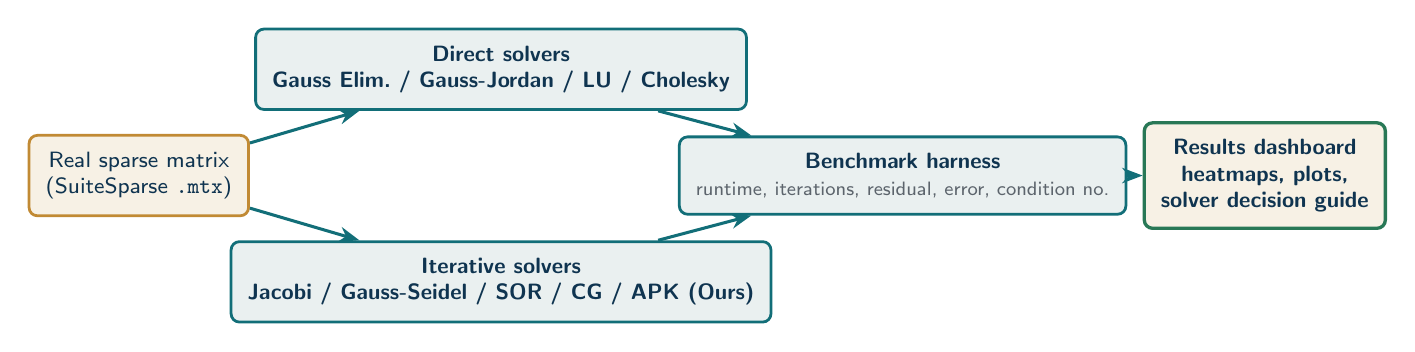
\begin{tikzpicture}
    \node[data] (in) at (0,0) {Real sparse matrix\\(SuiteSparse \texttt{.mtx})};
    \node[stage] (direct) at (4.6,1.35) {Direct solvers\\Gauss Elim.\ / Gauss-Jordan / LU / Cholesky};
    \node[stage] (iter) at (4.6,-1.35) {Iterative solvers\\Jacobi / Gauss-Seidel / SOR / CG / \textbf{APK (Ours)}};
    \node[stage] (bench) at (9.7,0) {Benchmark harness\subtag{runtime, iterations, residual, error, condition no.}};
    \node[outbox] (out) at (14.3,0) {Results dashboard\\heatmaps, plots,\\solver decision guide};
    \draw[fl] (in) -- (direct);
    \draw[fl] (in) -- (iter);
    \draw[fl] (direct) -- (bench);
    \draw[fl] (iter) -- (bench);
    \draw[fl] (bench) -- (out);
  \end{tikzpicture}}

  \vspace{0.9em}
  \small
  \begin{itemize}\setlength\itemsep{0.42em}
    \item \textbf{Ground truth:} generate a known $\vec{x}$, compute $\vec{b}=A\vec{x}$,
      solve with every method, measure the residual: fully deterministic, no
      ambiguity in what ``correct'' means.
    \item \textbf{Solvers evaluated:} benchmark classical textbook solvers alongside \textbf{our proposed novel method (APK)}.
    \item \textbf{Scale:} sweep across real engineering matrices, correlated against sparsity and condition number.
    \item \textbf{Payoff:} a concrete, evidence-based answer to ``which solver,
      for which real system'', the exact question every engineering simulation
      has to answer before it can even start.
  \end{itemize}
\end{frame}

%----------------------------------------------------------------- EXPANDED SCOPE
\begin{frame}{Expanded Scope: 26 Engineering Domains}
  \vspace{-0.15em}
  \colorbox{LSlightgold}{\parbox{0.98\linewidth}{\vspace{0.25em}
    {\bfseries\normalsize\color{LSnavy} Scaled Benchmark: 830 Real Matrices across 26 Scientific \& Engineering Domains}\\[0.18em]
    {\footnotesize\color{LSgray} Scaling up from the initial 48-matrix pilot to a massive dataset spanning $n = 5$ to $10{,}000$ unknowns.}
    \vspace{0.25em}}}
  \vspace{0.35em}

  \small
  \begin{columns}[T]
    \begin{column}{0.49\textwidth}
      \textbf{\color{LSteal}Core Engineering Domains:}
      \vspace{0.25em}
      \begin{itemize}\setlength\itemsep{0.25em}\footnotesize
        \item \textbf{Circuit Simulation} (200 systems): SPICE, VLSI interconnects, transient \& DC nodes.
        \item \textbf{Fluid Dynamics (CFD)} (126 systems): Navier-Stokes equations, aerodynamic flow.
        \item \textbf{Structural Mechanics} (87 systems): Stiffness \& mass matrices, FEM deformation.
        \item \textbf{Optimal Control \& Optimization} (117 systems): Trajectory planning, linear programming.
      \end{itemize}
    \end{column}

    \begin{column}{0.49\textwidth}
      \textbf{\color{LSteal}Scientific \& Physical Domains:}
      \vspace{0.25em}
      \begin{itemize}\setlength\itemsep{0.25em}\footnotesize
        \item \textbf{Chemical \& Quantum Chemistry} (75 systems): Reactor kinetics, molecular orbitals.
        \item \textbf{Electromagnetics \& Acoustics} (27 systems): Wave propagation, radar scattering.
        \item \textbf{Power Networks \& Thermal} (19 systems): Grid admittance, thermal diffusion.
        \item \textbf{Network Graphs \& Robotics} (55 systems): Directed/undirected graphs, kinematics.
      \end{itemize}
    \end{column}
  \end{columns}

  \vspace{0.35em}
  \begin{block}{\small Why Benchmarking 26 Real Domains Matters}
    \footnotesize Different physical domains produce fundamentally distinct matrix structures (symmetry, condition number $\kappa(A)$, diagonal dominance, and sparsity patterns). This multi-domain scale stress-tests solver stability and generalizability across real science.
  \end{block}
\end{frame}

%----------------------------------------------------------------- NOVELTY: APK METHOD
\begin{frame}{Our Proposed Novel Method: APK Solver}
  \vspace{-0.15em}
  \colorbox{LSlightgold}{\parbox{0.98\linewidth}{\vspace{0.25em}
    {\bfseries\normalsize\color{LSnavy} Our Contribution: Adaptive Preconditioned Krylov (APK) Solver}\\[0.15em]
    {\footnotesize\color{LSgray} Designed by our team to overcome the failure modes of classical solvers on complex physical systems.}
    \vspace{0.25em}}}
  \vspace{0.6em}

  \small
  \begin{itemize}\setlength\itemsep{0.75em}
    \item \textbf{\color{LSteal}Novel Multi-Stage Architecture:}
      Combines adaptive preconditioning, automated physics routing, and iterative defect correction into a single unified solver.

    \item \textbf{\color{LSteal}Adaptive Preconditioning Hierarchy:}
      Constructs multi-level Incomplete LU factorizations with automated fallbacks to diagonal scaling for ill-conditioned systems.

    \item \textbf{\color{LSteal}Dynamic Physics Dispatch:}
      Inspects matrix symmetry and definiteness in real time, routing symmetric positive-definite systems to PCG and unsymmetric systems to BiCGSTAB.

    \item \textbf{\color{LSteal}Iterative Defect Refinement:}
      Applies lightweight residual correction passes using the cached preconditioner, recovering precision up to machine epsilon.

    \item \textbf{\color{LSteal}Expected Advantage:}
      Provides a robust solver designed to handle ill-conditioned and unsymmetric systems where classical Jacobi, Gauss-Seidel, and CG diverge.
  \end{itemize}
\end{frame}

%----------------------------------------------------------------- ADDRESSING TEACHER FEEDBACK
\begin{frame}{Addressing Teacher Feedback}
  \vspace{-0.15em}
  \colorbox{LSlightgold}{\parbox{0.98\linewidth}{\vspace{0.25em}
    {\bfseries\normalsize\color{LSnavy} Systematic Performance \& Failure-Mode Analysis}\\[0.15em]
    {\footnotesize\color{LSgray} Moving beyond raw benchmark numbers to explain the mathematical root causes of solver behavior.}
    \vspace{0.25em}}}
  \vspace{0.5em}

  \small
  \begin{itemize}\setlength\itemsep{0.6em}
    \item \textbf{\color{LSteal}Which methods perform well (and when):}
      Identify which solvers achieve the best speed, accuracy, and stability for each specific domain and matrix structure.

    \item \textbf{\color{LSteal}Which methods fail (and where):}
      Examine and catalog exactly where solvers diverge, break down, or lose numerical precision across different physical systems.

    \item \textbf{\color{LSteal}Why methods succeed or fail:}
      Trace performance directly to underlying mathematical properties, including condition number $\kappa(A)$, symmetry, diagonal dominance, and sparsity.

    \item \textbf{\color{LSteal}Public Dataset \& Verification:}
      All 830 matrices are sourced from the public, standard SuiteSparse benchmark collection and pre-verified to be valid square real-valued systems.
  \end{itemize}
\end{frame}

%=============================================================================
%  UPDATE SLIDES -- results after the full benchmark, added after the proposal
%=============================================================================

\begin{frame}{Update: What the Full Benchmark Found}
  \vspace{-0.15em}
  \colorbox{LSlightgold}{\parbox{0.98\linewidth}{\vspace{0.25em}
    {\bfseries\normalsize\color{LSnavy} 930 matrices $\times$ 16 solvers $=$ 14{,}880 measurements}\\[0.15em]
    {\footnotesize\color{LSgray} 27 domains, $n = 5$ to $10{,}000$. Every result is scored by the
    harness from the residual it measures itself, never by a solver's own convergence flag.}
    \vspace{0.25em}}}
  \vspace{0.5em}
  \small
  \renewcommand{\arraystretch}{1.25}
  \begin{tabular}{@{}p{4.5cm}p{2.1cm}p{1.9cm}p{3.1cm}@{}}
    \toprule
    \hdrow \hdtxt{Solver} & \hdtxt{Applicable} & \hdtxt{Solved} & \hdtxt{Conditional success}\\
    \midrule
    \texttt{spsolve} (SuperLU) & 904 & \textcolor{LSgreen}{\textbf{876}} & 96.9\%\\
    \rowcolor{LSlight}
    Gauss elimination / LU & 598 & 595 & 99.5\%\\
    ILU-Krylov (dispatched) & 739 & 619 & 83.8\%\\
    \rowcolor{LSlight}
    Gauss-Seidel & 414 & 121 & 29.2\%\\
    Jacobi & 414 & 75 & 18.1\%\\
    \bottomrule
  \end{tabular}
  \vspace{0.6em}
  \begin{block}{\small Two numbers, never one}
    \footnotesize \emph{Applicability} is how much of the corpus a method is even defined on;
    \emph{conditional success} is how much of that it actually solves. Jacobi and Gauss-Seidel
    are undefined on \textbf{491 of 930} systems, because a zero on the diagonal leaves nothing
    to divide by.
  \end{block}
\end{frame}

\begin{frame}{Update: The APK Claim Does Not Survive}
  \small
  \vspace{0.2em}
  We proposed APK as a novel method. Measured against the baselines it was missing, the
  dispatch rule that made it ``ours'' contributes \textbf{one matrix}.
  \vspace{0.5em}
  \begin{center}
  \renewcommand{\arraystretch}{1.25}
  \begin{tabular}{@{}p{6.6cm}p{3.0cm}@{}}
    \toprule
    \hdrow \hdtxt{Configuration} & \hdtxt{Solved (of 739)}\\
    \midrule
    ILU-Krylov, symmetry dispatch \emph{(the proposal)} & 619\\
    \rowcolor{LSlight}
    ILU-BiCGSTAB, no dispatch at all & 618\\
    ILU only, zero Krylov iterations & 79\\
    \bottomrule
  \end{tabular}
  \end{center}
  \vspace{0.5em}
  \begin{itemize}\setlength\itemsep{0.3em}
    \item The dispatch rule is the decision flowchart in Barrett et al., \emph{Templates}
      (SIAM, 1994), and the default behaviour of PETSc and MATLAB's backslash.
    \item Its accuracy advantage came from an \textbf{iterative refinement pass no other
      method received}. Given the same pass, \textcolor{LSred}{\bfseries Jacobi} becomes the most
      accurate method in the benchmark: $6.99\times10^{-16}$ against APK's $7.11\times10^{-14}$.
    \item A sparse direct solver beats every iterative configuration: \textbf{876 against 619}.
  \end{itemize}
  \vspace{0.3em}
  {\footnotesize\color{LSgray} Reporting this is the point. A negative result we found ourselves
  is worth more than a claim a reviewer would break.}
\end{frame}

\begin{frame}{Update: Why the Base Paper's Effect Vanishes}
  \small
  On the 414 systems where both methods are defined: \textbf{75} both converge,
  \textbf{46} only Gauss-Seidel, and \gd{zero} only Jacobi, against the 1{,}095 only-Jacobi
  cases the base paper reports at $n \le 5$.
  \vspace{0.5em}
  \begin{center}
  \renewcommand{\arraystretch}{1.2}
  \begin{tabular}{@{}p{5.4cm}p{1.6cm}p{2.5cm}p{2.5cm}@{}}
    \toprule
    \hdrow \hdtxt{Hypothesis class} & \hdtxt{Systems} & \hdtxt{Jacobi works} & \hdtxt{Only-Jacobi}\\
    \midrule
    Strictly diagonally dominant & 43 & 88.4\% & 0\\
    \rowcolor{LSlight}
    H-matrix & 83 & 77.1\% & 0\\
    M-matrix & 34 & 64.7\% & 0\\
    \rowcolor{LSlight}
    \textbf{No theorem applies} & \textbf{192} & \textcolor{LSred}{\bfseries 1.6\%} & 0\\
    \bottomrule
  \end{tabular}
  \end{center}
  \vspace{0.55em}
  \begin{block}{\small A theorem can be true and still useless}
    \footnotesize Householder and John (1958) guarantee Gauss-Seidel converges for every
    symmetric positive-definite matrix, and $\rho(T_{GS}) < 1$ does hold on 98 of our 104 SPD
    systems. Within a 10{,}000-iteration budget it delivers on \textbf{44}: the remaining 54
    need a median of \textbf{1{,}798{,}184} iterations. That gap is invisible at $n \le 5$.
  \end{block}
\end{frame}

\begin{frame}{Update: Our Actual Contribution}
  \vspace{-0.15em}
  \colorbox{LSlightgold}{\parbox{0.98\linewidth}{\vspace{0.25em}
    {\bfseries\normalsize\color{LSnavy} Convergence-Oriented Diagonal Selection}\\[0.15em]
    {\footnotesize\color{LSgray} A stationary method divides by $a_{ii}$, so it depends entirely on
    which entries sit on the diagonal, and that was decided by the order the rows arrived in.}
    \vspace{0.25em}}}
  \vspace{0.5em}
  \small
  \begin{itemize}\setlength\itemsep{0.42em}
    \item \textbf{\color{LSteal}Most preprocessing provably cannot help.}
      Row scaling gives $T_J' = I - (RD)^{-1}RA = T_J$ exactly; column scaling is a similarity
      transform; a symmetric permutation leaves $\rho(T_J)$ invariant. \textbf{Only a row
      permutation changes which entries form $D$.}
    \item \textbf{\color{LSteal}MC64 optimises the wrong objective.}
      It maximises $\prod |a_{ii}|$, built for pivot stability in \emph{direct} solvers.
      Convergence instead needs a small row ratio $\sum_{j \ne i} |a_{ij}| / |a_{ii}|$.
    \item \textbf{\color{LSteal}We minimise the worst row ratio}, a bottleneck assignment solved
      by binary search plus bipartite matching. No single objective wins everywhere, so all
      candidates are computed and ranked by an estimated $\rho(T_{GS})$ in about $0.01$\,s.
  \end{itemize}
  \vspace{0.4em}
  \begin{center}
  \colorbox{LSlight}{\parbox{0.94\linewidth}{\centering\footnotesize
  \texttt{odepa400}: $\rho(T_{GS}) = 1.0001$ as given, MC64 leaves it unchanged,
  ours reaches \gd{$0.495$} and Gauss-Seidel converges.\\
  A shuffled $3\times3$: $\rho(T_{GS})$ falls from $99.19$ to $0.0316$, solved in 7 iterations.}}
  \end{center}
\end{frame}

\end{document}
